\documentclass[tikz, border=4pt]{standalone}
\usepackage{tikz}
\usepackage{tikz-cd}
\begin{document}
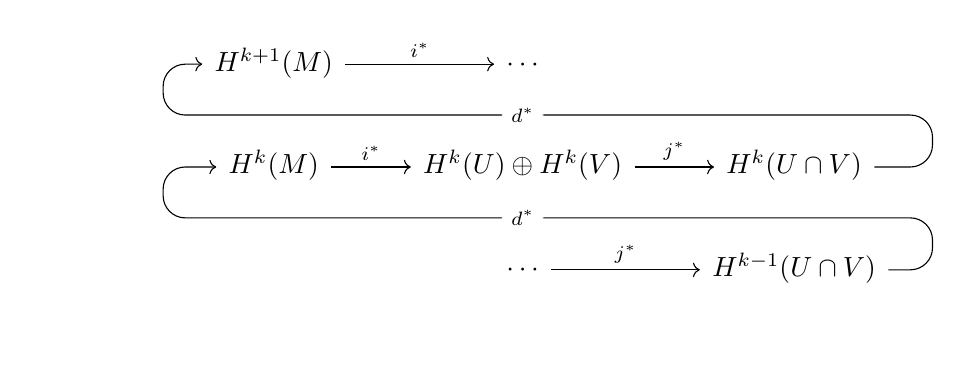
\begin{tikzpicture}[x=1cm, y=1cm]
  \node at (5.67,-1.96) {\pgfinterruptpicture%
  \tikzset{
  curarrow/.style={
  rounded corners=8pt,
  execute at begin to={every node/.style={fill=red}},
  to path={-- ([xshift=50pt]\tikztostart.center)
    |- (#1) node[fill=white] {$\scriptstyle d^*$}
    -| ([xshift=-40pt]\tikztotarget.center)
    -- (\tikztotarget)}
    }
  }
  \begin{tikzcd}[cells={nodes={text height=2ex,text depth=0.75ex}}]
    {} & & H^{k+1}(M) \arrow{r}{i^*} & \cdots \\
    {} & & H^k(M) \arrow{r}{i^*} & H^k(U) \oplus H^k(V) \arrow{r}{j^*}
    \arrow[draw=none]{u}[name=Y, shape=coordinate]{}
    \arrow[draw=none]{d}[name=Z,shape=coordinate]{}
    & H^k(U \cap V) \arrow[curarrow=Y]{ull}{} \\
    & & & \cdots \arrow{r}{j^*} & H^{k-1}(U \cap V)
    \arrow[curarrow=Z]{ull}{} \\
  \end{tikzcd}%
  \endpgfinterruptpicture};
\end{tikzpicture}
\end{document}
